\section{Pestaña para Importar del DOG}
\label{PBusquedaDOG}

\begin{figure}[H]
\centerline{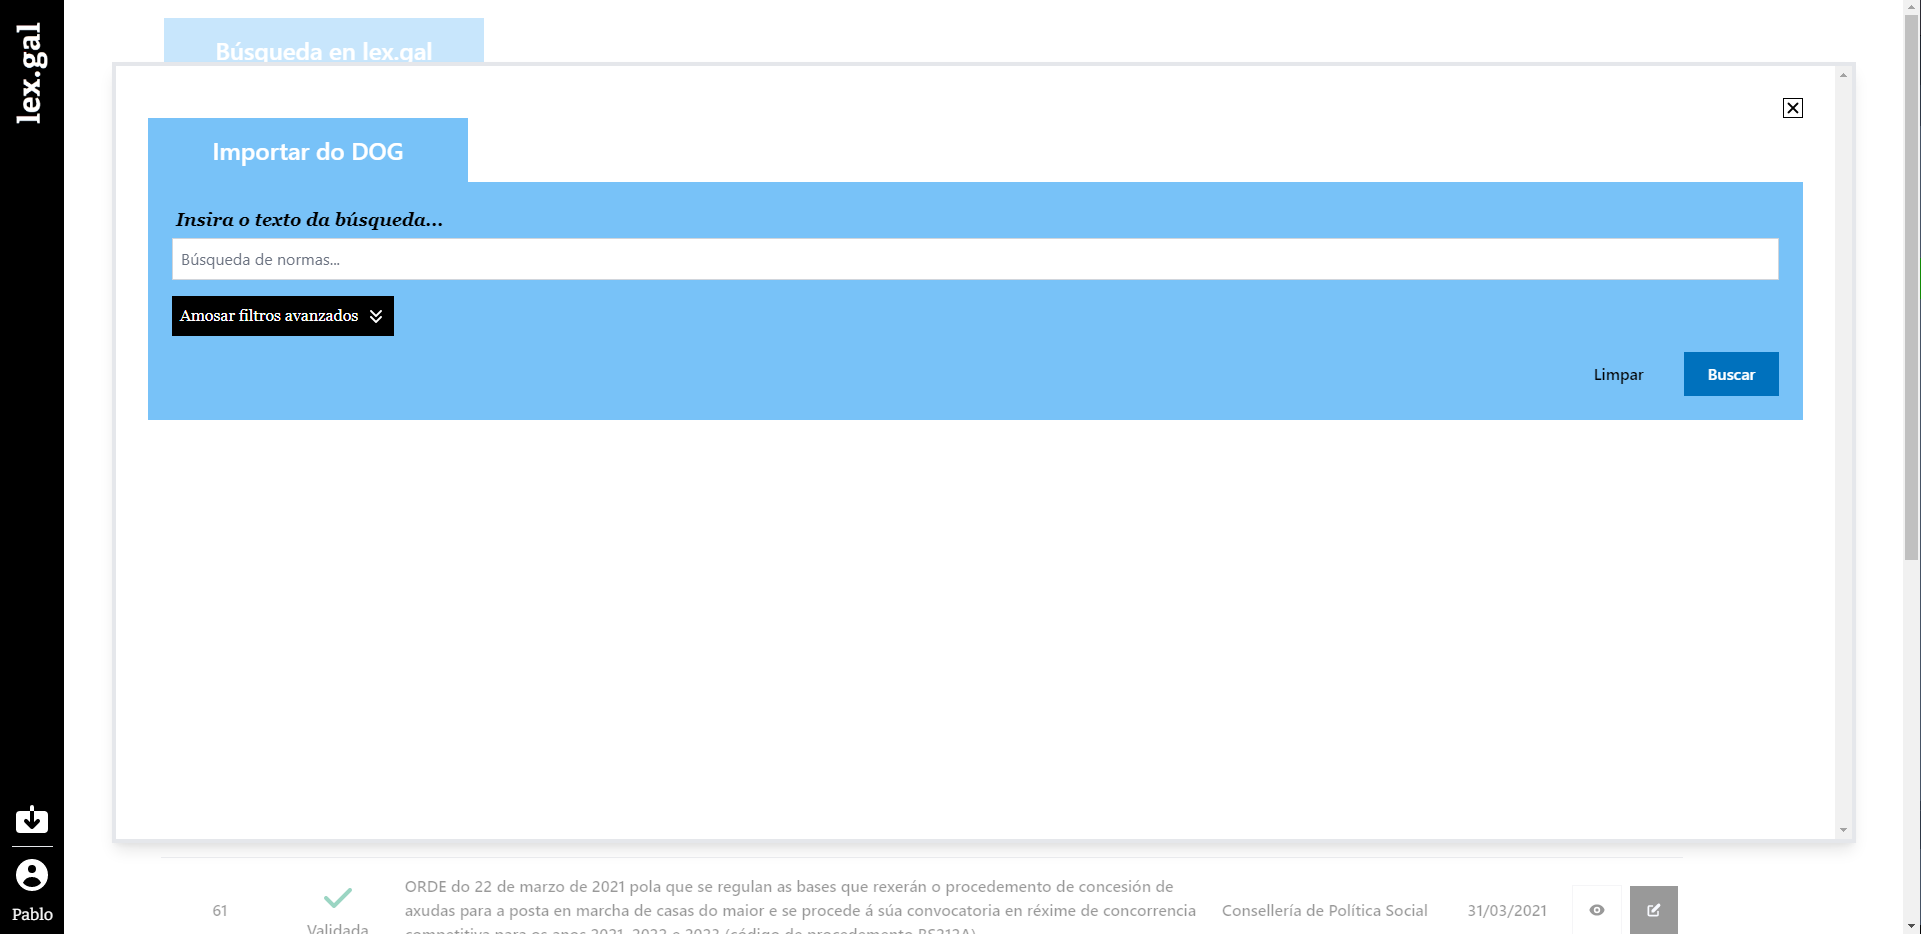
\includegraphics[width=12cm]{figuras/manualUsuario/BuscarDOG.PNG}}
\caption{Pestaña para importar del DOG - I.}
\label{enlacePBusquedaDOG}
\end{figure}

En esta pestaña se permite buscar leyes en el DOG. Al igual que en la búsqueda de la página principal, tenemos un campo de texto, un botón para limpiar el campo, y el propio botón de buscar. Si pinchamos en ``Amosar filtros avanzados'', se mostrarán una serie de filtros a la hora de realizar la búsqueda en el DOG.
\\

Una vez realizada la búsqueda, se deberá ver algo semejante a lo siguiente:

\begin{figure}[H]
\centerline{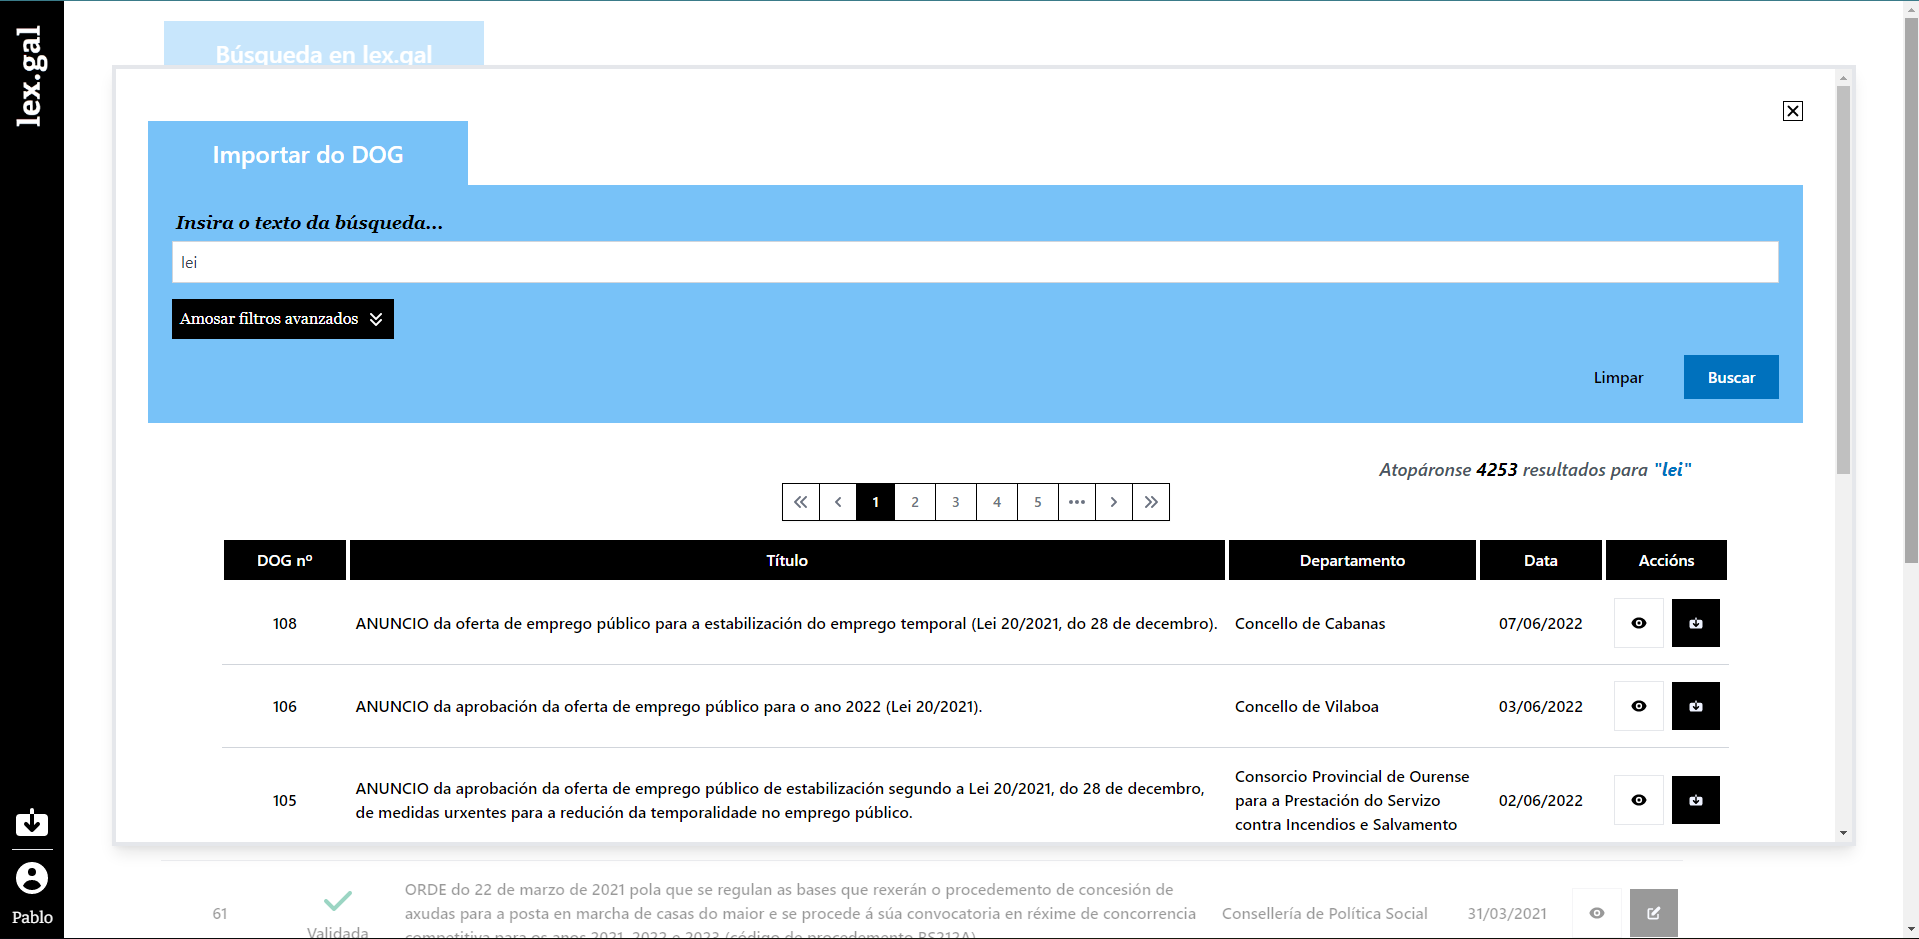
\includegraphics[width=12cm]{figuras/manualUsuario/BuscarDOGCompleta.PNG}}
\caption{Pestaña para importar del DOG - II.}
\label{enlacePBusquedaCDOG}
\end{figure}

En ella se muestra una tabla con las leyes del DOG encontradas, donde encontramos una serie de acciones por cada ley. Si se pincha en el botón del ojo, se podrá previsualizar la ley en el propio DOG, como se puede observar:

\begin{figure}[H]
\centerline{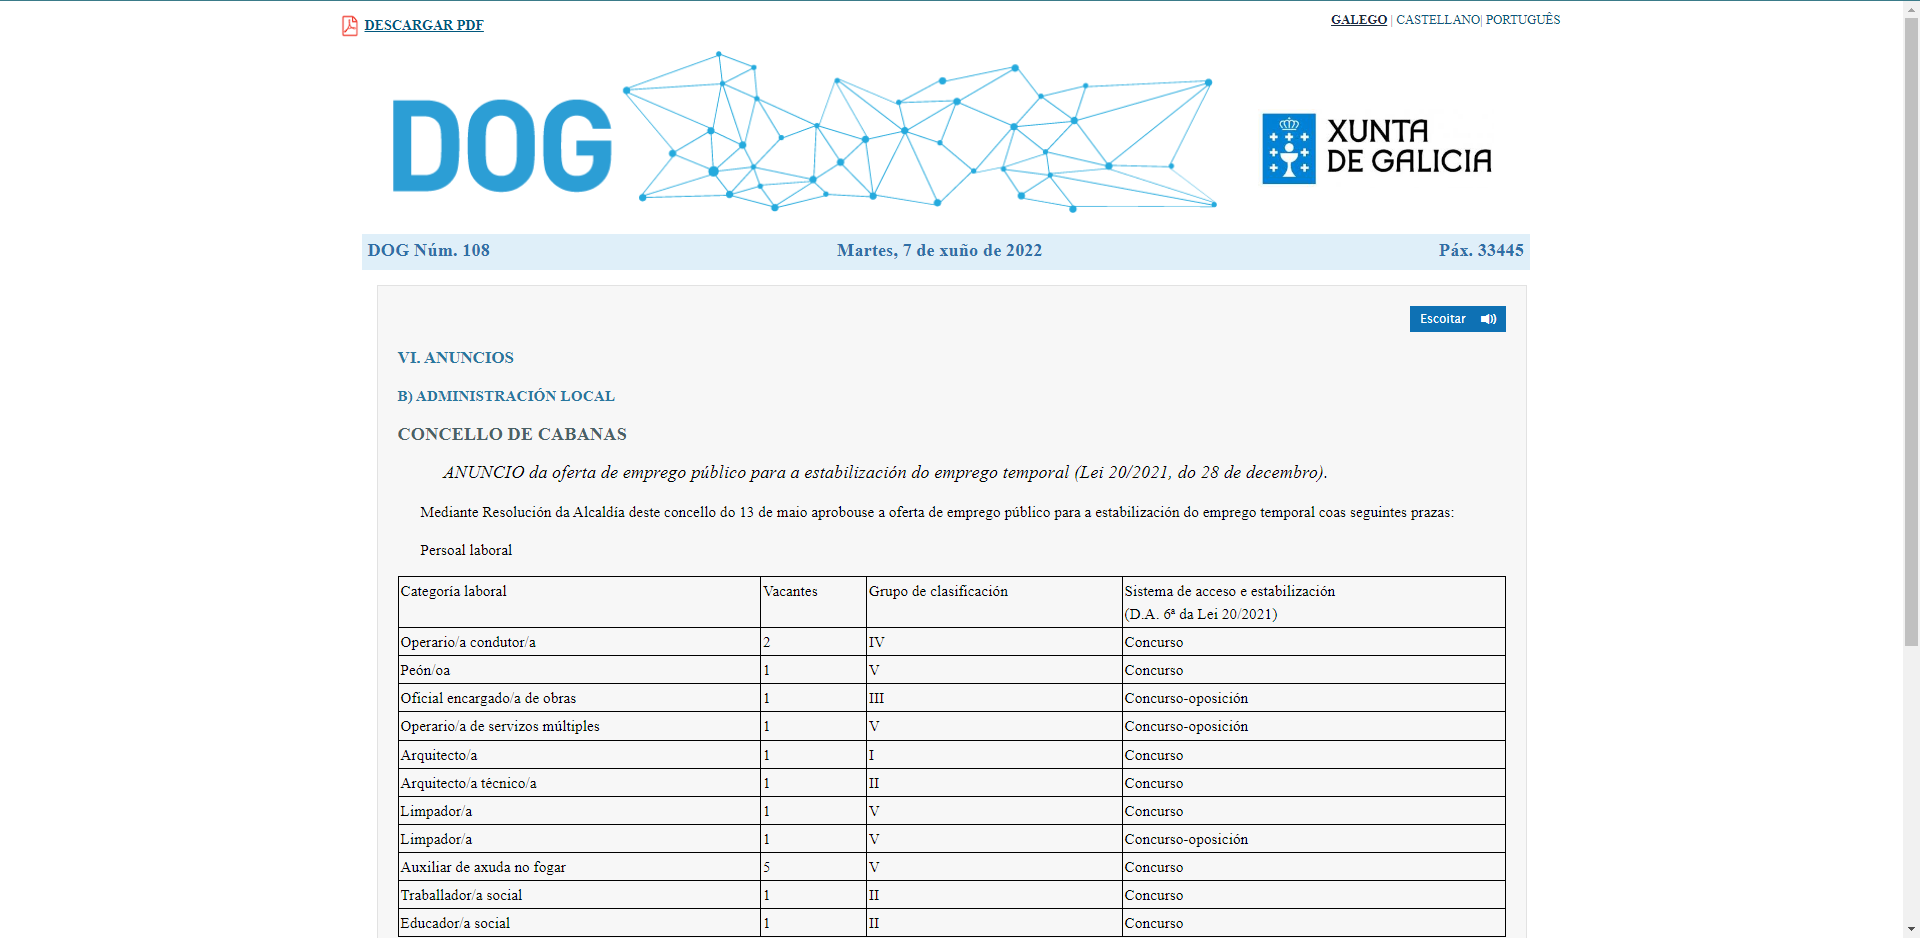
\includegraphics[width=12cm]{figuras/manualUsuario/PrevisualizarDOG.PNG}}
\caption{Previsualización de ley del DOG.}
\label{enlacePrevisDOG}
\end{figure}

En el caso de pinchar en el botón con una flecha hacia abajo, se importará una ley a la aplicación de lex.gal, pasando a estar disponible en la página principal del programa.

\section{Página de previsualización de una ley de lex.gal}
\label{PPrevisualizacionLexGal}

\begin{figure}[H]
\centerline{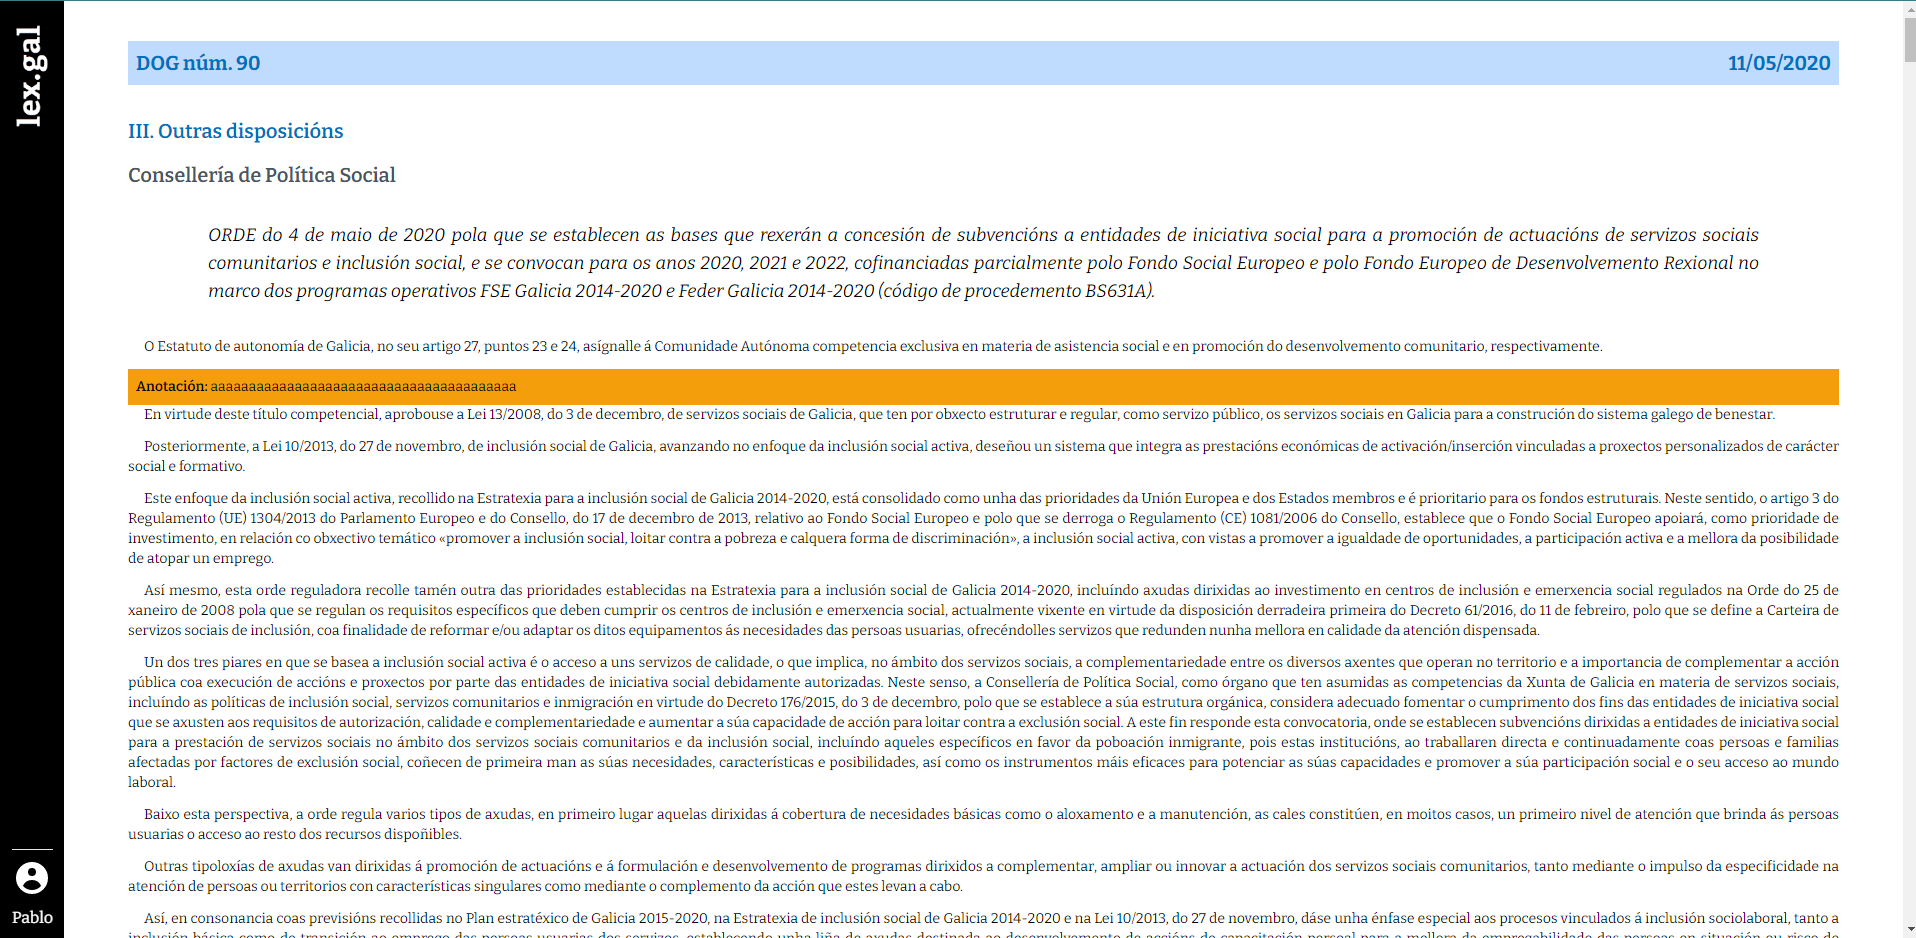
\includegraphics[width=15cm]{figuras/manualUsuario/PrevisualizarLEXGAL.PNG}}
\caption{Página de previsualización de una ley de lex.gal.}
\label{enlacePrevisualizacionLexGal}
\end{figure}

En esta página se puede previsualizar el contenido de una ley de lex.gal. Se mostrará en ella:
\begin{itemize}
    \item En el recuadro azul el número del DOG y la fecha de publicación en el DOG.
    \item Con color de letra azul el título de la sección a la que pertenece.
    \item Con color gris el publicador del documento.
    \item Con letra cursiva el título/sumario de la ley.
    \item En texto plano, el contenido de la propia ley.
    \item Con fondo naranja, las anotaciones realizadas sobre un párrafo de la ley.
\end{itemize}